\chapter{The Trinity Stones: History}

\begin{center}
	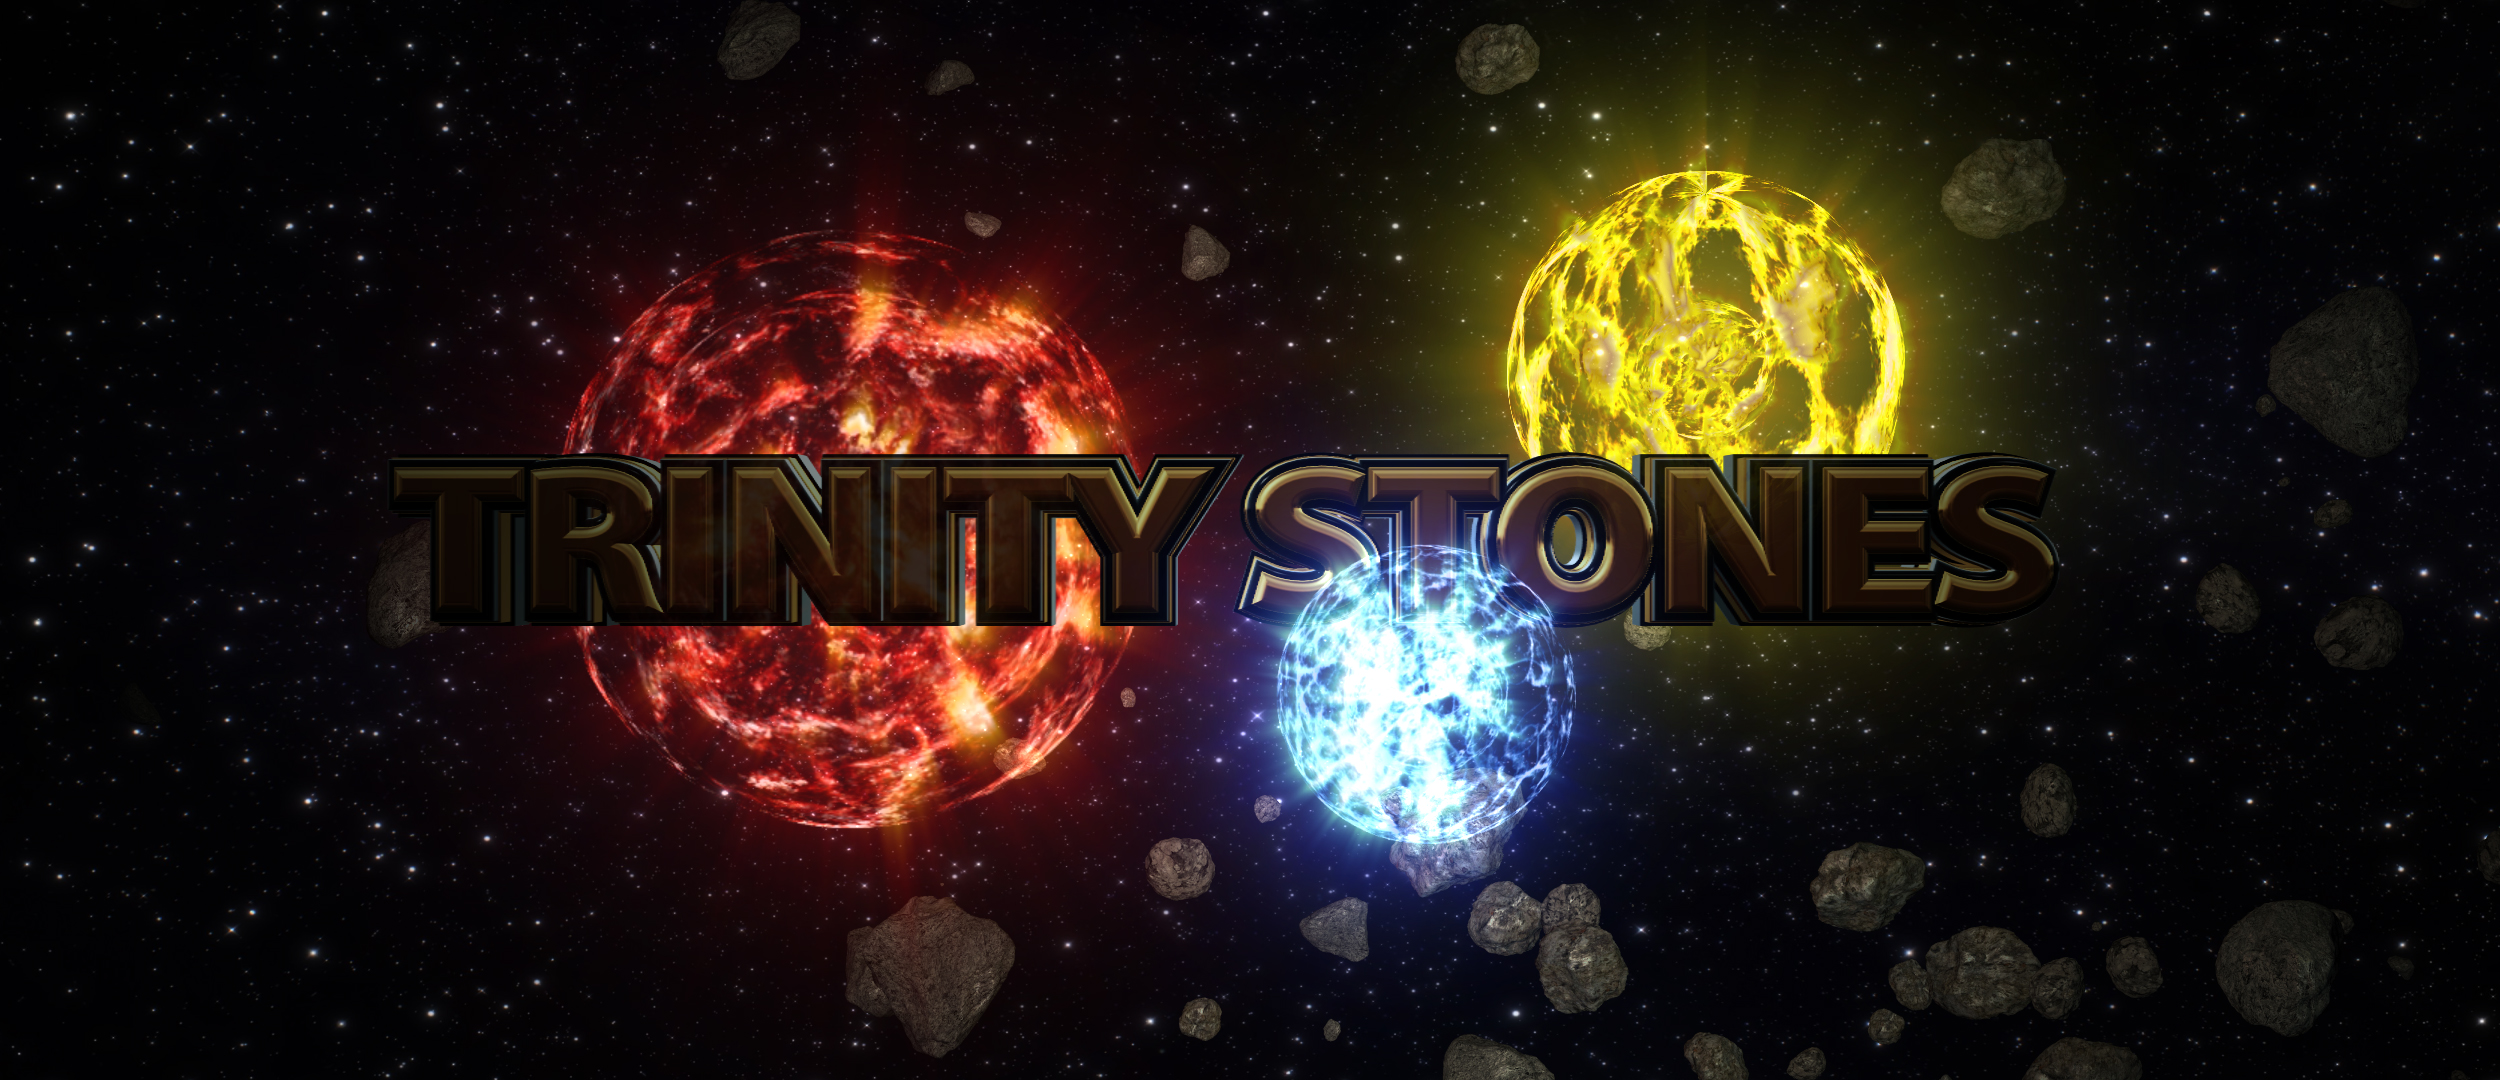
\includegraphics[width=\linewidth]{img/TS.jpg}
\end{center}


\section{Creation of a Trinity}

\begin{quotebox}
	In the beginning, The Celestials created the Heavens and the Earth. A singularity of reality from whence space was formed, energy was made, and time unraveled. A trinity of reality to be seen forever.
\end{quotebox}

No matter the story of beginning, it all arrives at the same principles. Space, time, and matter. A trinity of reality stemming from the creation itself. For none can exist without another, and in existence all must come simultaneously. These forces of the cosmos work in unison and cannot be broken from each other. At least that's how we've perceived it.

\section{Creation of the Stones}

\textbf{It is said} that those who can harness the power of reality itself would have unrivaled power. The outcomes of reality itself would be for them to decide. Unfortunately to harness the trinity would be to harness the universe, a space incomprehensible to perceive. In ancient times, there existed an organization known as the Celestial Guard. This group of people extended through all races and across the entire world. A common goal among them was to understand and tap into this trinity. Through centuries, hidden mysteries of the universe began to be unraveled, bringing forth the secrets of magic and powers known today. The Celestial Guard was the primary source of the advancements of knowledge. It is said that the knowledge and understandings of these ancients vastly surpassed anyone from todays era. 

Over time, the Celestial Guard became segregated. After discoveries pertaining to parallel realms, there became hidden agendas. A civil war on a global scale ensued among the Celestial Guard. A war on such great of a scale that the majority of knowledge was lost as a consequence. As it is told, the council of seven (the last leaders of the Celestial Guard) had unlocked an understanding that has never before been known. Through this they were able to create what we call the Infinity Stones. 

A minuscule part of reality was harnessed into three stones, space, time, and matter. Each stone is unique in appearance but all mesmerizing in appearance. The stones are said to bring immeasurable powers to the users. Not by their powers themselves, but through the understanding they bring. The stones were created as a milestone in understanding. Unfortunately, due to the war and the hastily actions of the council, the stones were hidden away. A powerful spell was placed on the stones such that they cannot be found save all together. If any stone is found apart from a counterpart, reality itself will bend around the stone, hence placing it back in hiding. 

The stones have a unique ability to act on their own each in a unique way. Each stone has a unique look which three sections. The stones are cut in such a way that they all fit together. The stones each have remnants of the others glow within it and parts of each stone will turn dark when the others are not near. 

\section{The Celestial Guard}

The legend of the Celestial Guard is an ancient world-wide coalition of beings. The Guard was started by a group of elite warriors whom banded together to dethrone a corrupt kingdom. Seven warriors in total were among the original Guard. They were able to take down an entire kingdom from within and established a new council of seven where their goals and actions carried enough wait to gain the allegiance of the masses. After establishing a new government, they created what was known as the Celestial Guard, where knowledge and understandings were all but the property of the world. 

Once established, the advancements of the era accelerated at a growing rate. This was before the time of wizards and sorcerers. However, through time, as secrets became unraveled, these classes became commonplace. Each generation, the council kept the same size of seven. Seven elite members based on their accomplishments. After a few hundred years, the council became involved with the discovery of the trinity of reality. The focus of the council's research became focused on this and this alone. Breakthroughs in this field lead to new spell discoveries and new ways to shape reality. Unfortunately the surface of knowledge was barely scratched, until one day.

In one era, a generation of six master sorcerers, wizards, and warlocks existed as part of the council. The seventh member was a warrior named Kurdran. It was rare that the whole council would get together, and just as rare for only six of them to get together. There was a find by one of the members, however, where all of the members got together save Kurdran. Together, the six members explored a new concept that one of them had discovered. After only a few short days, a rift in space was created. A single point in space was expanded and shown to contain energy and time in the absence of space (at least, the space that had been known about). This was the void. The six members were not prepared for what followed and one of them was lost to sealing the rift. This rift had unforeseen consequences throughout all of space. Space became unstable and rifts began to appear at random.

This incident created changes on a global scale, which negatively impacted the incentives of many. New possibilities in magic were being opened to many. The council was now down to six total. Somehow, through a chain of small events, news got out of the council and rumors were put together with the new changes that the rift brought. The council was blamed and civil war broke out. This was a war to drown out all other wars. The war went on for years, between new factions that had broken out within the Celestial guard. The six council members appeared to have all dissipated. In reality, they were hidden. With the opening of the void, plane shifting was now an option. The council members banded together as six hidden in reality on a new plane. There they were able to focus on their studies. They believed the only way to reverse what they had done with the initial rift is to understand the other elements of the trinity. 

First, the council had to disrupt time itself, creating a reality of only space and matter. One mistake doing this and they would have been trapped in a single moment for eternity. Following this, matter had to be torn from reality to 
create existence pertaining of only space and time. A pure vacuum in which anything matter would be instantly annihilated. With each advancement, reality itself became more unstable. It took much time, but after learning what they could about these new realities, they knew how to stop the chaos. This is when the Trinity Stones were created. The stones were containers for the tears in our reality. They each bear the power of the trinity to seal each individual tear in reality.

Among returning from hiding, the world was shattered. While away, the void realm had consumed many, time had been warped, energy expanded out of balance. The trinity stones ended the chaos, but the damage was irreparable. The Celestial Guard was no longer a thing, for the members had all been scattered, destroyed, or changed. The stones were then sealed away, behind a powerful spell. The last act of the council before they disbanded. The members each went their own way in order aid and rebuild in different locations. Over time, the Celestial Guard was forgotten by most. The world grew into a new place as it is today and all of this only exists in mere legend.  

\section{The Space Stone}

The space stone controls elements pertaining to spacial events. The space stone mainly causes objects to randomly move location.


\section{The Matter Stone}

The matter stone controls elements pertaining to power and lack thereof. The matter stone primarily causes illusionary events such as glowing ponds and rivers as well as transforms beasts into both stronger or weaker than they usually would be.

\section{The Time Stone}

The time stone controls temporal events. The stone primarily will cause objects to teleport into different locations within the flow of time.

\section{The Celestials}

The reality of the Myths laid by the Trinity Stones follow from an Ancient sect developed from the Celestial Guard. The understandings brought about by the age of the celestial guard lead to greater understandings of consciousness\footnote{The Ideas for this are from Stargate SG-01} and the infinite universe. The world was not thrown into chaos like legend claims but rather destroyed by its own inhabitants a millennium later. Within a few thousand years of research and after the creation of the stones and understandings brought about from the multidimensional discoveries of the time, a sect of beings discovered a way of shedding their spirits from their physical bodies and existing on a higher plane of existence. 

This shedding of the soul was known as ascension and was seen by many as a way of ultimate understanding. Unfortunately some of these beings discovered there was a connection between the mortal souls and the ascended souls and in the mortals worshiped the ascended beings their power and understanding was enhanced. Others decided that with this existence as an ascended being, they do not have the right or purpose or need to affiliate with lower life forms and took off into the universe to gain a greater understanding. The ascended beings who stayed called themselves the celestials after the Celestial Guard and believed they had achieved the ultimate destiny and form of understanding. These beings looked at themselves as gods and thought it appropriate to rule over the lower beings.

The Celestials created a religion known as Celestas in which they had mortals worshiping them with the false hope of ascension. The religion was based on the Celestas Writings (or the Book of Celestas). Through time, the celestials convinced all of their followers that the unbelievers must be destroyed which inevitably lead to world wars. This lead to the destruction of almost the entire population and loss of most knowledge. The myth of the Trinity stones was preserved through a group of knights lead by Myrddin who was a member of a break off group from the Celestial Guard known as the Alterans. 

Through the power of the Celestials, they "enhance" individuals (priors of Celestas) to spread the word of Celestas throughout the lands. These priors cannot easily be defeated because they have powers pertaining to understandings from the Celestials that protect them. However, the priors are generally peaceful and only harm via the armies they command. They will send themselves in if something really needs done but mainly stick to preaching while their armies are off conquering. After the destruction of the world, many centuries went by as the Celestas followers rebuilt their population as well as the rest of the planet did too.

The Book of Celestas refers to the day of the Lamb, which is a prophesied day of conquest through all of Orilla. To fulfill this conquest, they have a three-fold plan (PFS - pestilence, famine, sword) that they use in the various regions and locations. The basic plan can be outlined by the below steps and is only deviated from in unique or rare situations.
\begin{enumerate}
	\item Send in a prior for one day/night to give word of the Celestials and perform miracles that are outlined in the Book of Celestas.
	\item Leave the area and after approximately a week, a plague starts to appear on the people. This plague spreads to the food and water thus appearing as though that is how it's transmitted. This leads to a famine in the land.
	\item Next, the prior returns after a few weeks with some of his followers.
	\item The prior then performs miracles to solve the issue of the plague and famine and attempts to convert all of the people as believers. If they are converted he will leave followers there to teach the people in how to worship and live in the Celestial lifestyle. If they do not want to be converted, the prior will say "Hallowed bin de Celestas. Herem die LOCATION" (Where LOCATION is the place/region in question). This statement containing "herem" means to utterly destroy in the name of the gods and is an order to purge the area.
	\item The army is sent in to takeover if they reject the ways of Celestas.
\end{enumerate}

\section{Myrddin}

Myrddin was an Alteran. His name, Myrddin can also be translated to Merlin, regarding Merlin and the knights of the round table. Merlin was a member of the Celestial guard whom figured out the secrets to ascension but saw the negative consequences it could have on the planet and universe. He decided to not ascend himself and instead rebelled against the Celestials. In doing so, none of the other Alterans (the ones who could ascend) stayed with Merlin and he was left alone with his beliefs. Myrddin was one of the first to determine the secrets behind ascension and was one of the most knowledgeable of people at that time.

Myrddin put it upon himself to create a technology allowing him to destroy ascended beings, which was not thought possible. However, he could not do such a thing outright because the Alterans and Celestials would have interfered and destroyed him, but instead he had to find a way to mask his work by shifting himself between dimensions. He was able to create a device known as the San'graal (The Holy Grail) which had the capabilities of destroying the Celestials but was unable to activate it due to him closely being watched by the Celestials. Myrddin instead left his work hidden behind secrets, like the Trinity stones and kept his secrets safe guarded by the knights of the round table throughout the generations.

Myrddin's end research was left in a secret lab which can only be accessed via the Trinity stones. Myrddin froze himself in stasis within his lab and he contains the knowledge of how to create the San'graal by it's base particles. If the Trinity Stones are fitted together (after being found of course), the users will be transported to Myrddin's Laboratory. Myrddin and his various other labs were all location in the Pluvian Forest. One of such places is referred to as Avalon which is a place where him and his knights kept all of the treasures from that age.

\section{Morgana}

Morgana (also known as Morgen La Fey where La Fey means the fairy) was an Alteran from Myrddin's time. She was greatly opposed to Myrddin advancing his capabilities to combat ascended beings due to her plans to ascend herself. Unfortunately, due to herself convincing that Myrddin succeeded in creating the San'graal, she never ascended herself. She dedicated her life to studying the Trinity stones and to determine Myrddin's secrets to destroy the San'graal before ascending. However, during her lifetimes, she was able to understand the true threat that the Celestials posed and changed her mind to side with Myrddin. Myrddin was significantly more clever than Morgana and Morgana determined that there were safeguards around the San'graal preventing her from finding it. Due to this, she is lying in wait to assist those who can actually find it. 

\subsection{Morgana Lore in the Campaign}

Morgana, also known as Morgan the fairy was a powerful enchantress in the Arthurian legend. She was a goddess, a sorcerer, benevolent and related to King Arthur, as his magical savior and protector. In many of her iterations, she has potential for both good and evil. Her prominence increased over time and some sources portray her in a cyclical prose such as the Vulgate cycle. The Vulgate cycle ands dimension to the King Arthur tradition, and the birth of Merlin as the son of a devil who gained the ability to see future events after transforming into a prophet. The earliest account of her equates her with the isle of apples (Avalon). which is where Arthur was taken after being fatally wounded. These claim she was removed from goddess status and became a mortal but retained all her powers.

 

